\documentclass[10pt]{beamer}
\graphicspath{{../images/}}
\usepackage{array,mathtools}
\usepackage{scalerel}
\usepackage{cancel}

\newcommand{\longdiv}{\smash{\mkern-0.43mu\vstretch{1.31}{\hstretch{.7}{)}}\mkern-5.2mu\vstretch{1.31}{\hstretch{.7}{)}}}}
\newcolumntype{B}[1]{r*{#1}{@{\hspace{0.3em}}r}}
\title{IEEE-754}
\author{Junseo Shin}
\date{April 11, 2024}
\usetheme[progressbar=frametitle]{metropolis}
\def\titlepage{%
    \usebeamertemplate{title page}%<---
}
\begin{document}
% title slide
\maketitle
\begin{frame}
    \frametitle{Outline}
    \begin{itemize}
        \item Introduction
        \item Floating Point Arithmetic
        \item Simulations and Examples
    \end{itemize}
\end{frame}
\section{Introduction}
\begin{frame}
    \frametitle{Should We Trust Computers?}
    \begin{itemize}
        \item The error in floating point as ``noise'' in the data.
        \item The computer automatically ``preprocesses" the data in a way that is not always what you
        want. 
    \end{itemize}
\end{frame}
\begin{frame}
    \frametitle{How does a computer operate on numbers?}
    \begin{align*}
        178956970 - 178957034  % \onslide<2->{-64}
    \end{align*} \vspace*{-\baselineskip}\pause
    \center $\Downarrow$
    \begin{figure}
        \centering
        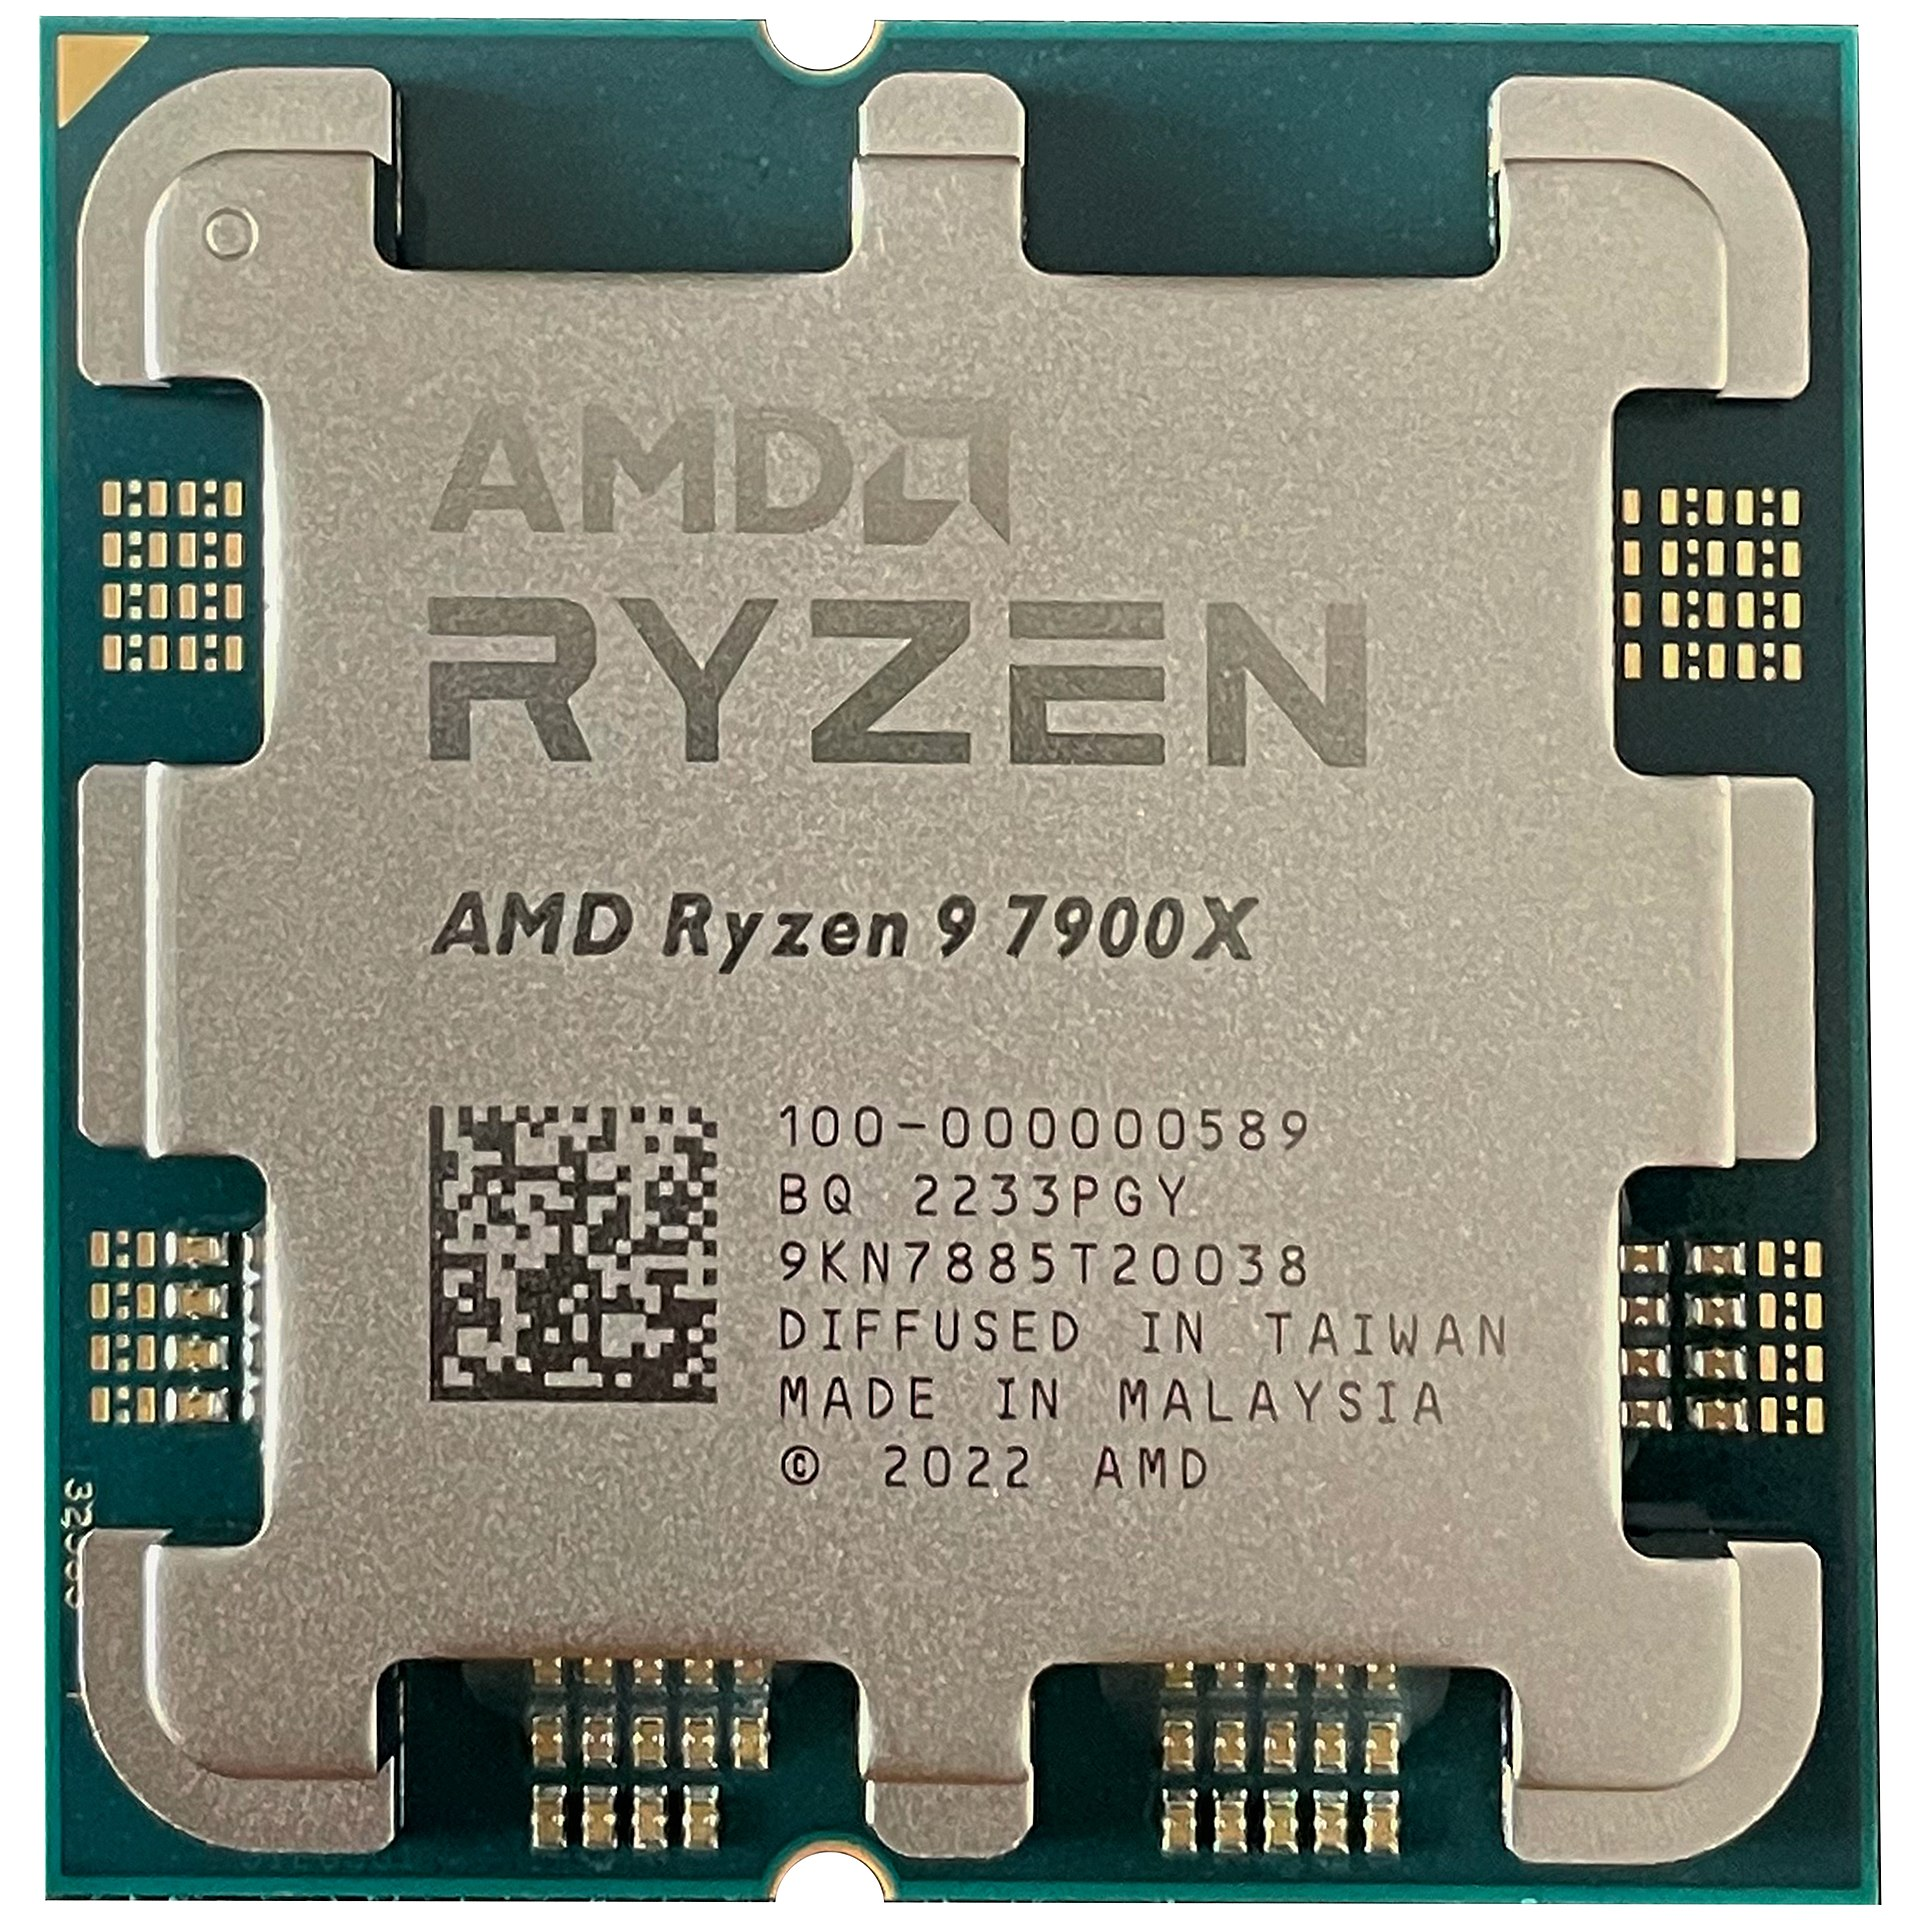
\includegraphics[width=0.3\textwidth]{ryzen9.png}
    \end{figure}
    \vspace*{-\baselineskip}\pause
    $\Downarrow$
    \begin{align*}
        = -64
    \end{align*}
\end{frame}

\begin{frame}
    \frametitle{Adding/Subtracting two 32 bit numbers}
    \begin{align*}
    \begin{array}{B8}
        (0)000 & 1010 & 1010 & 1010 & 1010 & 1010 & 1010 & 1010 \\
        {} - (0)000 & 1010 & 1010 & 1010 & 1010 & 1010 & 1110 & 1010 \\\hline
        (1)000 & 0000 & 0000 & 0000 & 0000 & 0000 & 0100 & 0000 
    \end{array}
\end{align*}
    \pause
    \begin{align*}
        = -2^6 = -64
    \end{align*}
\end{frame}

\begin{frame}
    \frametitle{Multiplying two binary numbers}
    % Shift and add method
    \begin{align*}
        170 \times 170 = 28900
    \end{align*}
    \pause
    \begin{align*}
        \begin{array}{cccccccccccccccc}
                &&&&&&&& 1 & 0 & 1 & 0 & 1 & 0 & 1 & 0 \\
          &&&&&&&\times& 1 & 0 & 1 & 0 & 1 & 0 & 1 & 0 \\
            \cline{8-16}
               &&&&&&&& 0 & 0 & 0 & 0 & 0 & 0 & 0 & 0 \\
                &&&&&&& 1 & 0 & 1 & 0 & 1 & 0 & 1 & 0 & \\
                 &&&&&& 0 & 0 & 0 & 0 & 0 & 0 & 0 & 0 &&\\
                  &&&&& 1 & 0 & 1 & 0 & 1 & 0 & 1 & 0 &&\\
                   &&&& 0 & 0 & 0 & 0 & 0 & 0 & 0 & 0 &&\\
                    &&& 1 & 0 & 1 & 0 & 1 & 0 & 1 & 0 &&\\
                     && 0 & 0 & 0 & 0 & 0 & 0 & 0 & 0 &&\\
                      & 1 & 0 & 1 & 0 & 1 & 0 & 1 & 0 &&\\
            \hline
            & 1 & 1 & 1 & 0 & 0 & 0 & 0 & 1 & 1 & 1 & 0 & 0 & 1 & 0 & 0
        \end{array}
    \end{align*}
\end{frame}

\begin{frame}
    \frametitle{Dividing Two Binary numbers}
    % Long division
    \begin{align*}
        \arraycolsep=1pt
        \begin{array}{ccccccccccccccccc}
            &          &&&&&&&& 1 &0 &1& 0 & 1&0&1&0  \\
    \cline{2-17}
    10101010&\longdiv  & 1 & 1 & 1 & 0 & 0 & 0 & 0 & 1 & 1 & 1 & 0 & 0 & 1 & 0 & 0 \\
            &          & 1 & 0 & 1 & 0 & 1 & 0 & 1 & 0 &      \\
    \cline{3-10}
            &          & 0 & 0 & 1 & 1 & 0 & 1 & 1 & 1 & 1 & 1  \\
            &          &   &   & 1 & 0 & 1 & 0 & 1 & 0 & 1 & 0  \\
    \cline{5-12}
            &          &   &   & 0 & 0 & 1 & 1 & 0 & 1 & 0 & 1 & 0 & 0  \\
            &          &   &   &   &   & 1 & 0 & 1 & 0 & 1 & 0 & 1 & 0  \\
    \cline{7-14}
            &          &   &   &   &   & 0 & 0 & 1 & 0 & 1 & 0 & 1 & 0 & 1 & 0   \\
            &          &   &   &   &   &   &   & 1 & 0 & 1 & 0 & 1 & 0 & 1 & 0   \\
    \cline{9-16}
            &          &   &   &   &   &   &   & 0 & 0 & 0 & 0 & 0 & 0 & 0 & 0
        \end{array}
    \end{align*}
\end{frame}

\begin{frame}
    \frametitle{Problems with Binary Integers}
    No way to represent rational numbers \pause
    \begin{itemize}
        \item Division is not accurate
        \begin{align*}
            3 / 2 = 1.5 \to 101 / 10 = 1.\cancel{1} = 1
        \end{align*} \pause
        \item Real-Valued Functions (e.g. $\sin(x), e^{x}, \sqrt{x}$)
    \end{itemize}
\end{frame}
 
\section{IEEE-754: Floating Point Arithmetic}
\begin{frame}
    \frametitle{From Decimal to Floating Point}
    Scientific Notation: $n \times 10^m$
    \begin{itemize}
        \item $1234 = 1.234 \times 10^3$
        \item $0.01234 = 1.234 \times 10^{-2}$
    \end{itemize} \pause
    Floating Point: (sign, significand, exponent)
    \begin{align*}
        (-1)^s \times m \times 2^{e}
    \end{align*}
\end{frame}

\begin{frame}
    \frametitle{Converting Decimal to Floating Point}
    Decimal $\to$ Binary $\to$ Floating Point
    \begin{align*}
        7.45 &\to 7 + 0.45 \\
        &\to 111.01110011001100110011001100110011\dots \\
        \onslide<2->{
            &\overbrace{\boxed{+}}^{\text{sign}} \underbrace{1.1101 \dots}_{\text{significand}} \times 2^{\overbrace{\boxed{2}}^{\text{exponent}}}
        }
    \end{align*}
    1 bit for sign, 8 bits for exponent, 23 bits for significand
    \pause
    \begin{align*}
        \boxed{0} \boxed{1000\; 0001} \boxed{1101\; 1100\;1100\; 1100\; 1100\; 110} 0110\dots
    \end{align*}
    \begin{align*}
        (-1)^{0} \times 2^{129 - 127} \times 1.1101\;1100\;1100\;1100\;1100\;110
    \end{align*}
\end{frame}

\begin{frame}
    \frametitle{Error in Floating Point}
    Machine Epsilon
    \begin{align*}
        \epsilon = 2^{-(p - 1)}
    \end{align*}
    \begin{itemize}
        \item Single Precision: $p = 24$: $\epsilon = 2^{-23} \approx 1.19 \times 10^{-7}$
        \begin{align*}
            1 + \epsilon = 1.0000\;0000\;0000\;0000\;0000\;001
        \end{align*}
        \item Double Precision: $p = 53$: $\epsilon = 2^{-52} \approx 2.22 \times 10^{-16}$
    \end{itemize}
\end{frame}

\section{Simulations and Examples}
\begin{frame}
    \frametitle{Python Example}
    % python terminal example 0.3 + 0.1
    \begin{figure}
        \centering
        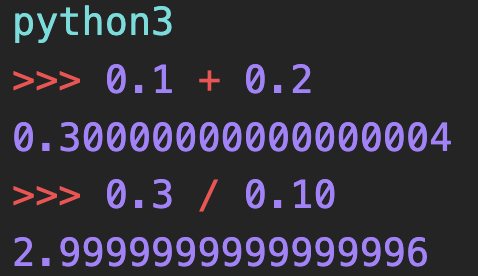
\includegraphics[width=0.8\textwidth]{pythoneg.png}
    \end{figure}
\end{frame}
\begin{frame}
    \frametitle{Simulating Larger Precision}
    GNU Multiple Precision Arithmetic Library (GNU MPFR)
    \begin{itemize}
        \item Used in Mathmatica
        \item Follows IEEE-754 standard but with arbitrary precision
        \item Does this solve the problem?
    \end{itemize}
\end{frame}
\begin{frame}
    \frametitle{Stirling's Approximation vs Factorial}
    % Insert picture of graph
    \begin{align*}
        n! &\approx \sqrt{2\pi n} \left(\frac{n}{e}\right)^n
    \end{align*}
    \pause
    Python Default (Float64, $p=53$) vs MPFR $(p = 100)$
    \begin{itemize}
        \item $n = 171 \to $ Overflow in Float64
        \item At $n = 100$, Fractional Error of $0.000833$ for both!
        \item Fractional Error of $10^{-6}$ at $n = 83334$ 
    \end{itemize}
\end{frame}
\begin{frame}
    \frametitle{Float64 vs MPFR}
    \begin{figure}
        \centering
        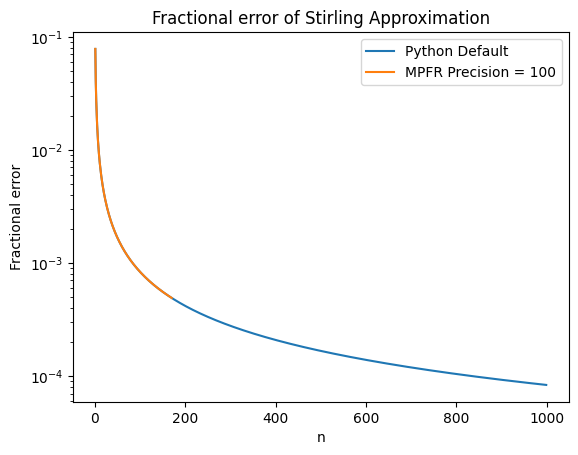
\includegraphics[width=0.8\textwidth]{fractional_error.png}
    \end{figure}
\end{frame}

\begin{frame}
    \frametitle{Patriot Defense Missile Failure}
    \begin{itemize}
        \item February 25, 1991: Patriot missile defense system failed to intercept SCUD missile
        \item 28 soldiers died
    \end{itemize}
\end{frame}

\begin{frame}
    \frametitle{Simulating Precision Loss}
    Converting Integer to 24 bit Floating Point
    \begin{itemize}
        \item Integer to 24 bit floating point: 1 sign bit, 8 exponent bits, 15 + 1 significand bits
        \item 100 hours or 360,000 seconds $\to 0\;10010001\; 010111111001000$
        \begin{align*}
            (-1)^0 \times 2^{145 - 127} \times 1.01111111001000 = 360,000
        \end{align*}
        \item 360,010 seconds $\to$ 360,000 seconds
    \end{itemize}
\end{frame}

\begin{frame}
    \frametitle{Simulating Precision Loss}
    \begin{itemize}
        \item Clock Speed: 10 ticks per second
        \begin{align*}
            0.1 \to 0.0999755859375
        \end{align*}
        Calculated time: 359912.109375
        \item Machine Epsilon $\epsilon = 2^{-20}$;
        Propogated Error $= \epsilon * \text{seconds}$
    \end{itemize}

\end{frame}
\begin{frame}
    \frametitle{Government Report}
    \begin{figure}
        \centering
        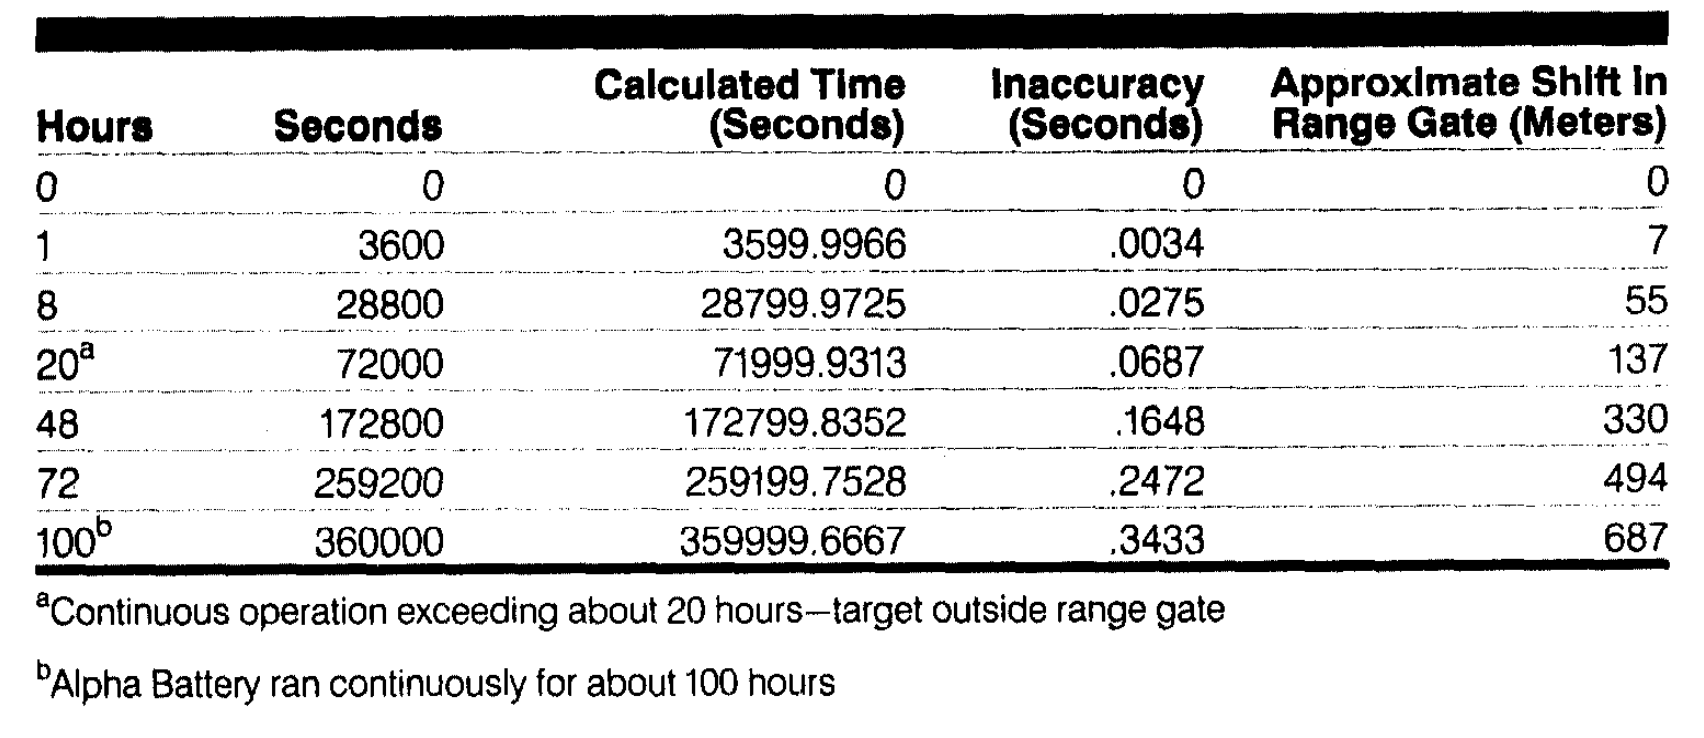
\includegraphics[width=1.0\textwidth]{patriot.png}
    \end{figure}
    [3]
\end{frame}

\begin{frame}
    \frametitle{Takehomes}
    \begin{itemize}
        \item You don't need to open a black box to understand where it fails
        \item Think about the limitations of a system. Just because it works in one instance doesn't mean it will work in another.
        \item Measure noise before you measure signal
    \end{itemize}
\end{frame}
\begin{frame}
    \frametitle{Reference}
    % link clickable in the pdf
    \bibliographystyle{plain}
    \bibliography{refs.bib}
    \cite{Goldberg_1991}
    \cite{8766229}
    \begin{itemize}
        \item \color{cyan}\href{https://floating-point-gui.de/}{https://floating-point-gui.de/}
        \item \href{https://www.gao.gov/products/imtec-92-26}{Patriot Missile Defense Software Problem Led to System Failure at Dhahran, Saudi Arabia [3]}
        \item \href{https://www.h-schmidt.net/FloatConverter/IEEE754.html}{Floating Point Converter}
    \end{itemize}
\end{frame}
\begin{frame}
    \frametitle{xkcd}
    \begin{figure}
        \centering
        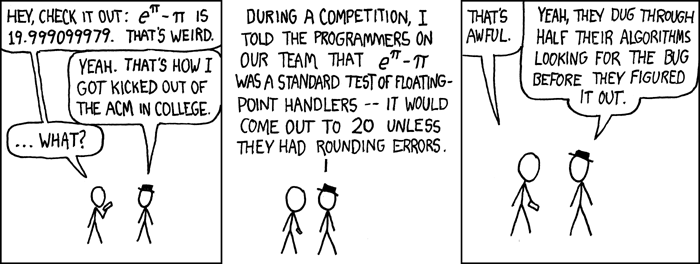
\includegraphics[width=0.8\textwidth]{xkcd.png}
    \end{figure}
    24 Bit Floating Point
    \begin{align*}
        e^\pi - \pi = 19.9970703125
    \end{align*}

    \href{https://xkcd.com/217/}{https://xkcd.com/217/}
\end{frame}
\end{document}